% !TEX root = report.tex

\subsection{Input file}

Now let's have a look at the input file.

First we see the first input file \texttt{inp1}, with $4$ \ce{Ar} atoms in a FCC cell,
the atom mass is assumed to be \SI{36.0}{\atomicmassunit},
see Fig. \ref{fig:fcc1} for reference.

\begin{figure}[h]
  \begin{minipage}{0.48\textwidth}
    \centering
    \input{Run/Tikz/FCC1}
    \caption{A FCC conventional unit cell of \ce{Ar} for \texttt{inp1}.}
    \label{fig:fcc1}
  \end{minipage}
\hfill
  \begin {minipage}{0.48\textwidth}
  \centering
  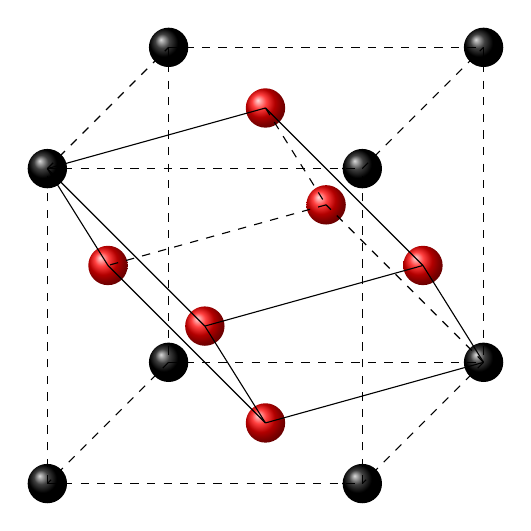
\begin{tikzpicture}
 %points on cube
 \coordinate (A) at (0,0,0);
 \coordinate (B) at (0,0,4);
 \coordinate (D) at (0,4,0);
 \coordinate (C) at (0,4,4);
 \coordinate (E) at (4,0,0);
 \coordinate (F) at (4,0,4);
 \coordinate (H) at (4,4,0);
 \coordinate (G) at (4,4,4);

 %center of faces
 \coordinate (I) at (0,2,2); %center of face ABCD
 \coordinate (J) at (4,2,2); %center of face EFGH
 \coordinate (K) at (2,4,2); %center of face DCGH
 \coordinate (L) at (2,0,2); %center of face ABFE
 \coordinate (M) at (2,2,4); %center of face CBGF
 \coordinate (N) at (2,2,0); %center of face DAEH

 %place non-atom cube corners
 \shade [ball color= black] (A) circle (0.25cm);
 \shade [ball color= black] (C) circle (0.25cm);
 \shade [ball color= black] (F) circle (0.25cm);
 \shade [ball color= black] (H) circle (0.25cm);
 \shade [ball color= black] (B) circle (0.25cm);
 \shade [ball color= black] (D) circle (0.25cm);
 \shade [ball color= black] (E) circle (0.25cm);
 \shade [ball color= black] (G) circle (0.25cm);

 %draw the center of each face
 \shade [ball color= red] (I) circle (0.25cm);
 \shade [ball color= red] (J) circle (0.25cm);
 \shade [ball color= red] (K) circle (0.25cm);
 \shade [ball color= red] (L) circle (0.25cm);
 \shade [ball color= red] (M) circle (0.25cm);
 \shade [ball color= red] (N) circle (0.25cm);

 %draw cube
 \draw [dashed] (A) -- (B);
 \draw [dashed] (B) -- (C);
 \draw [dashed] (C) -- (D);
 \draw [dashed] (D) -- (A);
 \draw [dashed] (E) -- (F);
 \draw [dashed] (F) -- (G);
 \draw [dashed] (G) -- (H);
 \draw [dashed] (H) -- (E);
 \draw [dashed] (A) -- (E);
 \draw [dashed] (B) -- (F);
 \draw [dashed] (C) -- (G);
 \draw [dashed] (D) -- (H);
 
 %draw unit cell
 \draw (E) -- (L);
 \draw (E) -- (J);
 \draw [dashed] (E) -- (N);
 \draw (J) -- (M);
 \draw (L) -- (M);
 \draw (J) -- (K);
 \draw [dashed] (K) -- (N);
 \draw (K) -- (C);
 \draw (M) -- (C);
 \draw (L) -- (I);
 \draw [dashed] (N) -- (I);
 \draw (C) -- (I);
\end{tikzpicture}

  \caption{A FCC primitive unit cell of \ce{Ar} for \texttt{inp3}, with
  face-center atoms filled in red.}
  \label{fig:fcc3}
\end{minipage}
\end{figure}

Run the simulation code, we derive the following results,
see Fig. \ref{fig:input1} for reference.
\begin{figure}[h]
 \centering
 \begin{minipage}[t]{0.45\textwidth}
  \includegraphics[width=\linewidth]{input1/avec_abc}
  \subcaption{Lattice parameters of \texttt{inp1}. The dashed dot lines are upper and lower
   bound of the lattice parameters. We can see that $a$, $b$, $c$ lines coincide with each
  other.}
  \label{fig:input1:avec}
 \end{minipage}
 \hfil
 \begin{minipage}[t]{0.45\textwidth}
  \includegraphics[width=\linewidth]{input1/t}
  \subcaption{Total energy of \texttt{inp1}. The dashed dot lines are upper and lower
   bound of the total kinetic energy and total potential energy. Total energy is the sum
  of the other two.}
  \label{fig:input1:e}
 \end{minipage}
 \hfil
 \vfill
 \begin{minipage}[t]{0.45\textwidth}
  \includegraphics[width=\linewidth]{input1/a}
  \subcaption{Atomic contribution to total energy of \texttt{inp1}.
   The dashed dot lines are upper and lower bound of the
   total atomic energy. We can see that atoms do not contribute
  to total kinetic energy.}
  \label{fig:input1:a}
 \end{minipage}
 \hfil
 \begin{minipage}[t]{0.45\textwidth}
  \includegraphics[width=\linewidth]{input1/l}
  \subcaption{Lattice contribution to total energy of \texttt{inp1}.
   The dashed dot lines are upper and lower bound of the
   total lattice energy. We can see that lattice do not contribute
  to total potential energy.}
  \label{fig:input1:l}
 \end{minipage}
 \caption{Simulation results for \texttt{inp1}.}
 \label{fig:input1}
\end{figure}

If we keep all other simulation parameters the same, but change
the size of time steps to $100$ in \texttt{inp2} (\texttt{inp1} is $200$) in Rydberg-like units,
i.e., decrease step size by a half, the results will be shown in Fig. \ref{fig:input2}.
There is not much differences from the first results. But looking in detail,
we can see that the amplitude of atomic potential in Fig. \ref{fig:input2:a} is not decaying
and the amplitude of lattice kinetic energy in Fig. \ref{fig:input2:l} is also not decaying
comparing to the corresponding figures Fig. \ref{fig:input1:a} and Fig. \ref{fig:input1:l},
respectively. And also, the amplitude of lattice parameter is not decaying in 
Fig. \ref{fig:input2:avec} rather than in \ref{fig:input1:avec}. We should also be aware of
that the oscillation frequency of energies, including kinetic and potential, do not change
as the time step is decreased to $\frac{ 1 }{ 2 }$, we will discuss later on this phenomenon.
\begin{figure}[h]
  \begin{minipage}[t]{0.45\textwidth}
    \includegraphics[width=\linewidth]{input2/avec_abc}
    \subcaption{Lattice parameters of \texttt{inp2}.}
    \label{fig:input2:avec}
  \end{minipage}
  \hfil
  \begin{minipage}[t]{0.45\textwidth}
    \includegraphics[width=\linewidth]{input2/t}
    \subcaption{Total energy of \texttt{inp2}.}
    \label{fig:input2:t}
  \end{minipage}
  \hfil
  \vfill
  %\vspace*{0.5cm} % (or whatever vertical separation you prefer)
  \begin{minipage}[t]{0.45\textwidth}
    \includegraphics[width=\linewidth]{input2/a}
    \subcaption{Atomic contribution to total energy of \texttt{inp2}.}
    \label{fig:input2:a}
  \end{minipage}
  \hfil
  \begin{minipage}[t]{0.45\textwidth}
    \includegraphics[width=\linewidth]{input2/l}
    \subcaption{Lattice contribution to total energy of \texttt{inp2}.}
    \label{fig:input2:l}
  \end{minipage}
  \caption{Simulation results for \texttt{inp2}.}
  \label{fig:input2}
\end{figure}

For \texttt{inp3}, now we shrink the unit cell size to $\frac{ 1 }{ 4 }$ of the
\texttt{inp1} and \texttt{inp2}, i.e., there is only $1$ \ce{Ar} atom in the 
cell. Also, the time step is $100$, the same as \texttt{inp2}.
See Fig. \ref{fig:fcc3} for reference.
Now let's see what will happen to the simulation result. see Fig. \ref{fig:input3}
for reference.
However, this time, the oscillation frequency of energies and lattice parameters
both increase by a factor of $2$, this is not astonishing because from 
$\eqref{eq:hdd}$ we know that 
\begin{equation}
  \omega \propto \sqrt{ 
 \frac{ B }{ W V } 
 },
\end{equation}
where $B$ is the bulk modulus.
Here we again see the decaying phenomenon,
comparing to simulation of \texttt{inp1}, we see that the oscillation amplitude of
both 
\begin{figure}[h]
  \begin{minipage}[t]{0.45\textwidth}
    \includegraphics[width=\linewidth]{input3/avec_abc}
    \subcaption{}
    \label{fig:input3:avec_abc}
  \end{minipage}
  \hfil
  \begin{minipage}[t]{0.45\textwidth}
    \includegraphics[width=\linewidth]{input3/t}
    \subcaption{}
    \label{fig:input3:t}
  \end{minipage}
  \hfil
  \vfill
  %\vspace*{0.5cm} % (or whatever vertical separation you prefer)
  \begin{minipage}[t]{0.45\textwidth}
    \includegraphics[width=\linewidth]{input3/a}
    \subcaption{}
    \label{fig:input3:a}
  \end{minipage}
  \hfil
  \begin{minipage}[t]{0.45\textwidth}
    \includegraphics[width=\linewidth]{input3/l}
    \subcaption{}
    \label{fig:input3:l}
  \end{minipage}
  \caption{\texttt{inp3}.}
  \label{fig:input3}
\end{figure}

